Das OOP Design Pattern \textbf{Observer} ermöglicht dynamische Verbindungen zwischen den einzelnen 
Objecten im Programm, um über die geschehenen Ereignisse im Programm alle Interessenten 
zu informieren.

Das Pattern besteht aus 2 Teilen: \textbf{Publisher} und \textbf{Observers} oder \textbf{Subscribers}

\textbf{Subscribers} können bestimmte Events des \textbf{Publishers} abonnieren und deabonnieren. 
Der \textbf{Publisher} informiert alle auf das geschehene Event abonnierten \textbf{Subscribers}, bzw. wenn es auftritt. 
Den \textbf{Subscribers} kann im Falle des Eintretens des Events ein gewisses Verhalten definiert werden.


\begin{figure}[H]
    \centering
    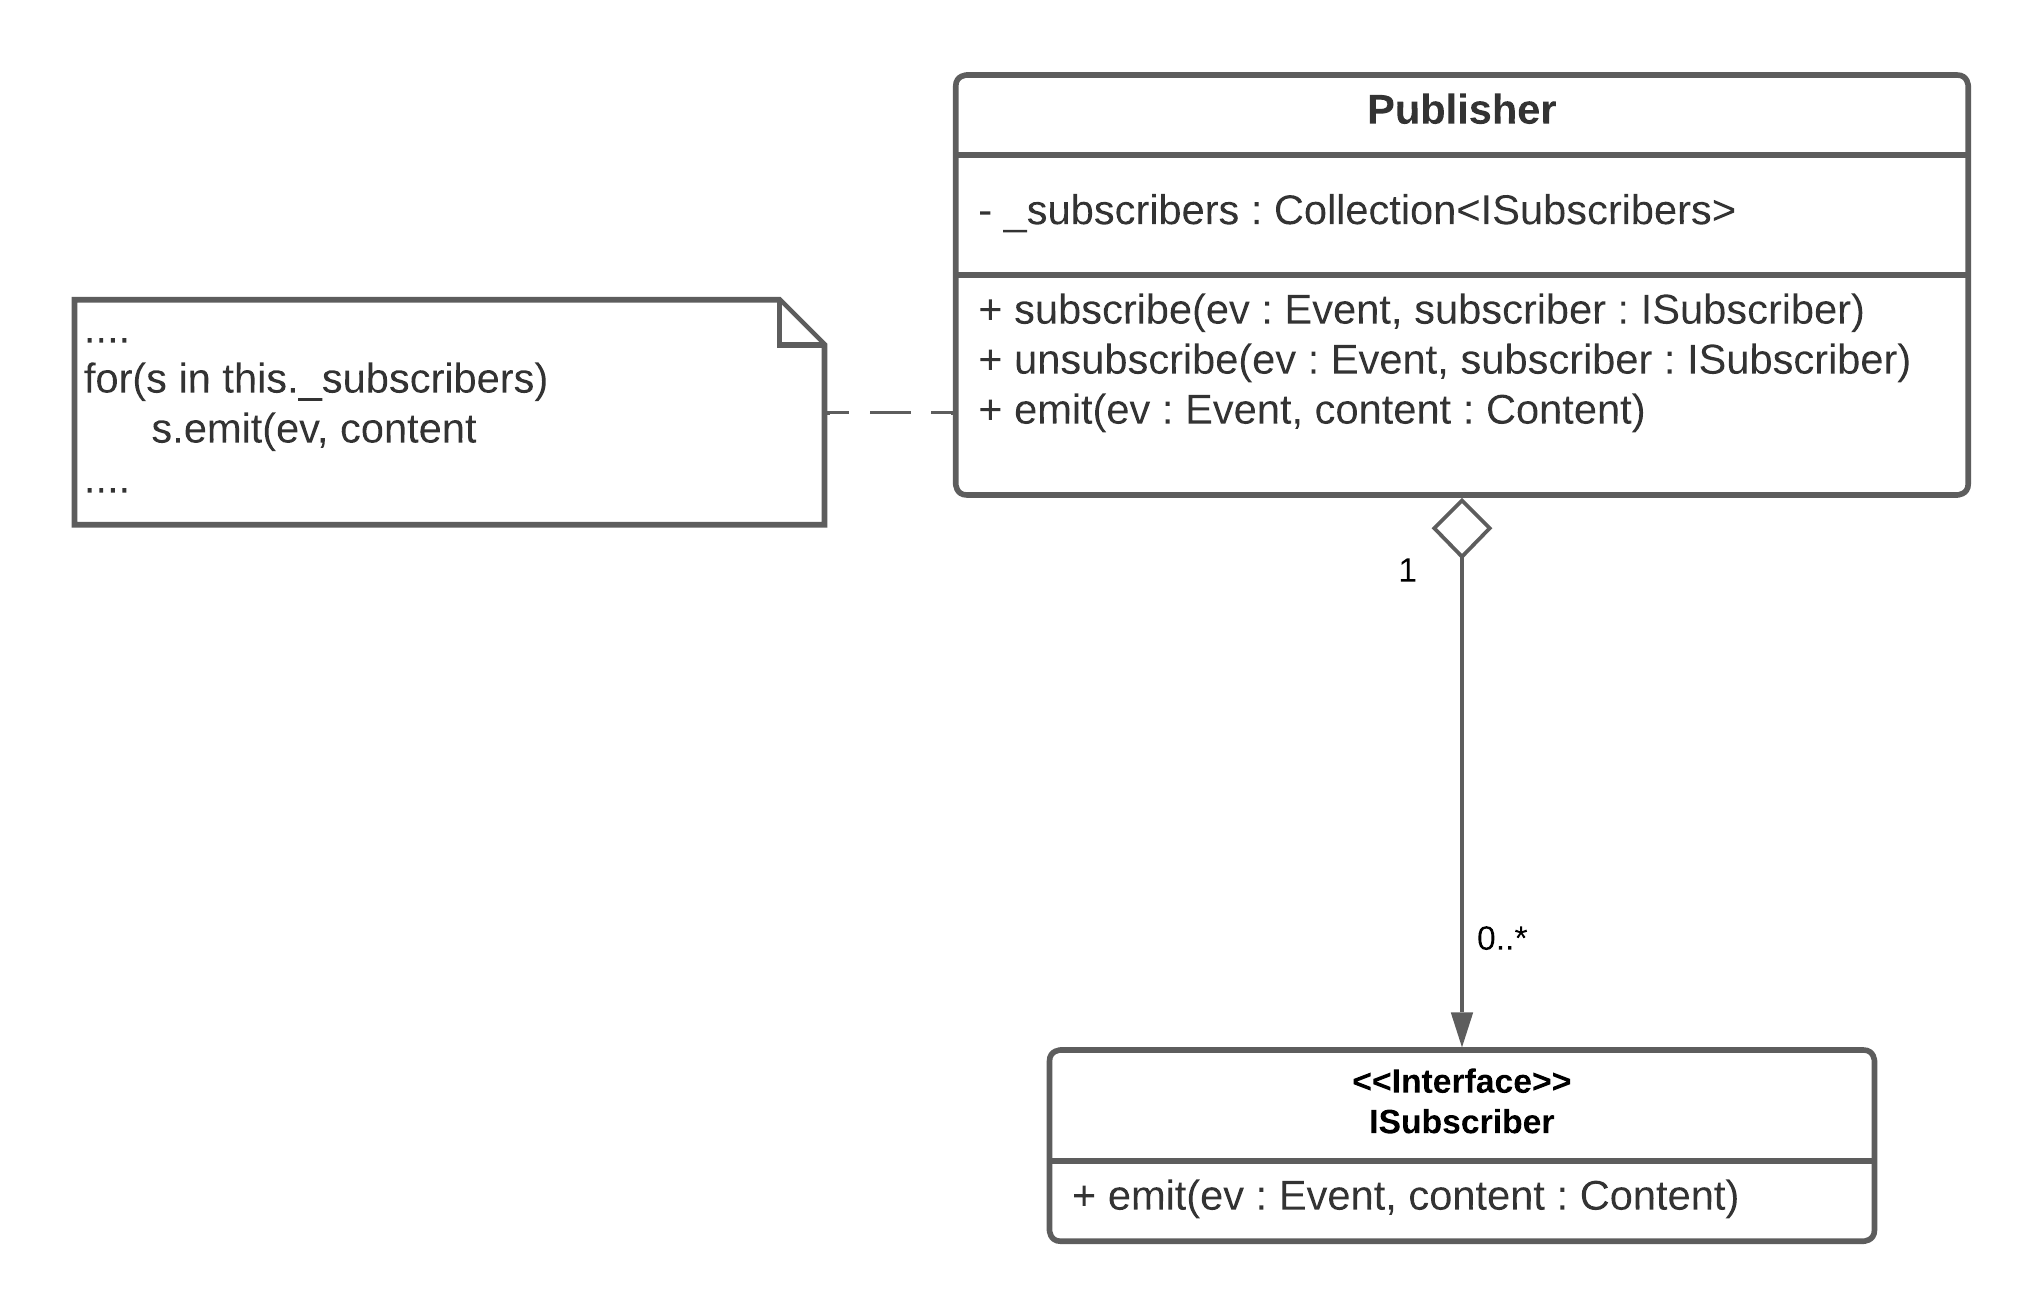
\includegraphics[width=1\textwidth]{Images/Observer.png}
    \caption[UML Observer]{Klassendiagrammm Observer}
    \label{fig:flow around cylinder}
    \source{Eigene Quelle}
\end{figure}